\part{Laboratory Session 07}
\section{Introduction}
In this session everything was prepared to put the BalanBot into operation. Unfortunately all BalanBots were already borrowed when everything was ready.

\section{System Initialization}
First the MPU6050 has to be initialized. This was done using $I^2C$ communication.
A value was assigned to the individual registers at the slave address 0x68.
For example, register 0x19 was assigned the value 7. So the sample rate was set with the formula:\\
	\begin{equation}
		1000Hz - \frac{8000Hz}{n-1}
	\end{equation}
In this formula n was replaced by the 7.	

\todo{Priority???}\\
\todo{Listings l�schen???}

	\begin{figure}[H]
		\centering
		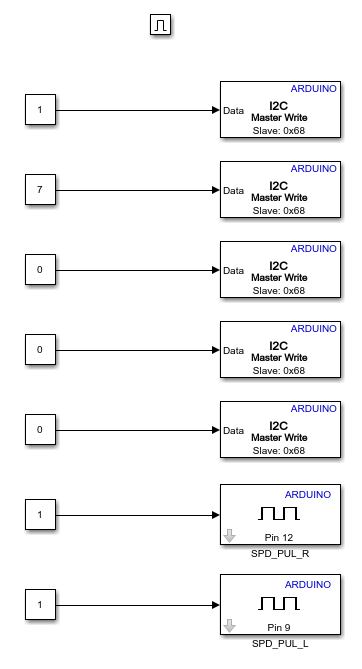
\includegraphics[width=0.25\textwidth]{figures/init.PNG}
		\caption{The initialization}	
		Source: Own presentation	
		\label{fig:init}	
	\end{figure}

	\begin{mdframed}
		\begin{lstlisting}[caption={C-Code from the script}, language=c,label={lst:init}]
	i2cData[0] = 7; // Set the sample rate to 1000Hz - 8kHz/(7+1) = 1000Hz
	i2cData[1] = 0x00; // Disable FSYNC and set 260 Hz Acc filtering, 256 Hz Gyro filtering, 8 KHz sampling
	i2cData[2] = 0x00; // Set Gyro Full Scale Range to +-250deg/s
	i2cData[3] = 0x00; // Set Accelerometer Full Scale Range to +-2g
	while (i2cWrite(0x19, i2cData, 4, false)); // Write to all four registers at once
	while (i2cWrite(0x6B, 0x01, true)); // PLL with X axis gyroscope reference and disable sleep mode		
		\end{lstlisting}
	\end{mdframed}
	
	\todo{L�schen?????}
	\begin{mdframed}
		\begin{lstlisting}[caption={Automatic generated C-Code from the model}, language=c,label={lst:init_real}]
	/* Start for Enabled SubSystem: '<Root>/One_time_initialization' */
	/* Constant: '<S1>/Constant1' */
	framework_I2CWrite4_Start(&framework_DW.I2CWrite);
	
	/* Constant: '<S1>/Constant2' */
	framework_I2CWrite4_Start(&framework_DW.I2CWrite1);
	
	/* Constant: '<S1>/Constant3' */
	framework_I2CWrite4_Start(&framework_DW.I2CWrite2);
	
	/* Constant: '<S1>/Constant4' */
	framework_I2CWrite4_Start(&framework_DW.I2CWrite3);
	
	/* Start for MATLABSystem: '<S1>/I2C Write4' incorporates:
	*  Constant: '<S1>/Constant5'
	*/
	framework_I2CWrite4_Start(&framework_DW.I2CWrite4);
	
	/* Start for MATLABSystem: '<S6>/Digital Output' */
	framework_DW.obj_g.matlabCodegenIsDeleted = true;
	framework_DW.obj_g.isInitialized = 0;
	framework_DW.obj_g.matlabCodegenIsDeleted = false;
	framework_DW.objisempty_f = true;
	framework_DW.obj_g.isSetupComplete = false;
	framework_DW.obj_g.isInitialized = 1;
	digitalIOSetup(12, true);
	framework_DW.obj_g.isSetupComplete = true;
	
	/* Start for MATLABSystem: '<S5>/Digital Output' */
	framework_DW.obj_lq.matlabCodegenIsDeleted = true;
	framework_DW.obj_lq.isInitialized = 0;
	framework_DW.obj_lq.matlabCodegenIsDeleted = false;
	framework_DW.objisempty_e1 = true;
	framework_DW.obj_lq.isSetupComplete = false;
	framework_DW.obj_lq.isInitialized = 1;
	digitalIOSetup(9, true);
	framework_DW.obj_lq.isSetupComplete = true;
	
	/* End of Start for SubSystem: '<Root>/One_time_initialization' */	
	
	/* Terminate for Enabled SubSystem: '<Root>/One_time_initialization' */
	framework_I2CWrite4_Term(&framework_DW.I2CWrite);
	framework_I2CWrite4_Term(&framework_DW.I2CWrite1);
	framework_I2CWrite4_Term(&framework_DW.I2CWrite2);
	framework_I2CWrite4_Term(&framework_DW.I2CWrite3);
	
	/* Terminate for MATLABSystem: '<S1>/I2C Write4' */
	framework_I2CWrite4_Term(&framework_DW.I2CWrite4);
	
	/* Terminate for MATLABSystem: '<S6>/Digital Output' */
	matlabCodegenHandle_matlabCod_f(&framework_DW.obj_g);
	
	/* Terminate for MATLABSystem: '<S5>/Digital Output' */
	matlabCodegenHandle_matlabCod_f(&framework_DW.obj_lq);
	
	/* End of Terminate for SubSystem: '<Root>/One_time_initialization' */		
		\end{lstlisting}
	\end{mdframed}

	

\section{Read Gyro Sensor Data}\label{sec:read}
	\begin{figure}[!htbp]
		\centering
		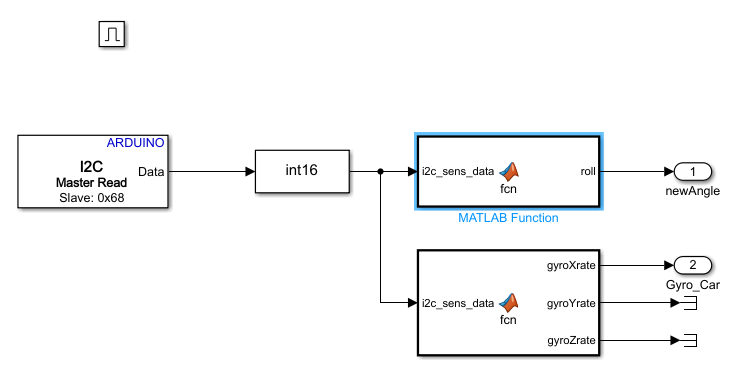
\includegraphics[width=0.7\textwidth]{figures/read.PNG}
		\caption{Processing of the read datas}	
		Source: Own presentation	
		\label{fig:read}	
	\end{figure}
The sensor data is processed in this block. First they are converted into the data type int16. 
Then the bus signal is splited into angle and gyro.
	\subsection{Angle}
	The Pythagorean theorem is used to calculate the absolute value of accX and accZ. With this value and accY the arctan finally calculates the angle in radians. At the end the angle is converted into degrees. Sown in Listing \ref{lst:roll}.
	\todo{Wieso wird seitliche Beschl accY ber�cksichtigt????}
		\begin{mdframed}
			\begin{lstlisting}[caption={Conversion from the acceleration to the angle}, language=matlab,label={lst:roll}]
			function roll = fcn(i2c_sens_data)
			accX = double(i2c_sens_data(1));
			accY = double(i2c_sens_data(2));
			accZ = double(i2c_sens_data(3));
			roll = atan(accY / sqrt(accX * accX + accZ * accZ)) * 180/pi;		
			\end{lstlisting}
		\end{mdframed}
	
	\subsection{Gyro}
	The data from the gyro sensor is converted to double format and then divided by 131. Shown in Listing \ref{lst:gyro}.
	\todo{why /131???}
		\begin{mdframed}
			\begin{lstlisting}[caption={Conversion to the gyros}, language=matlab,label={lst:gyro}]
			function [gyroXrate,gyroYrate,gyroZrate] = fcn(i2c_sens_data)
			gyroX = double(i2c_sens_data(5));
			gyroY = double(i2c_sens_data(6));
			gyroZ = double(i2c_sens_data(7));
			gyroXrate = gyroX/131;
			gyroYrate = gyroY/131;
			gyroZrate = gyroZ/131;	
			\end{lstlisting}
		\end{mdframed}
	
	\subsection{Test in External Mode}
	\todo{Was stellten wir fest}
	

\section{Controller}
The controller now uses the sensor data prepared in Section \ref{sec:read}. First, measurement errors are reduced with the kalman filter.
Then the filtered angle is converted into a PWM signal by a PID controller.
For the factors of the PID controller the values recommended in the script were taken first. These were finally adjusted by tests on the BalanBot. For this purpose, the simulation in Simulink was run in the external mode.\\
\todo{replace figure with update values and descripe the new Values}

	\subsection{Kp}
	xx
	\subsection{Ki}
	xx
	\subsection{Kd}
	xx
	
	\begin{figure}[H]
		\centering
		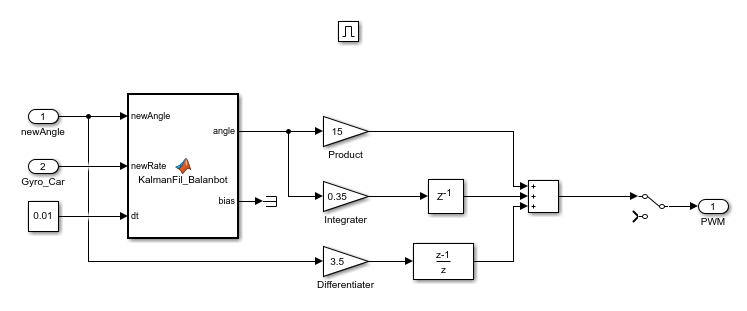
\includegraphics[width=0.7\textwidth]{figures/controller.PNG}
		\caption{Kalman Filter and PID Controller}	
		Source: Own presentation	
		\label{fig:controller}	
	\end{figure}


\section{Actuators}
The direction of rotation of the motors is done with an H-bridge of the digital outputs at pins 3, 4, 7 and 8. If the PWM input is greater than zero, the motors rotate in one direction. If it is smaller, they rotate in the other direction.
This PWM input value is finally converted into a PWM signal.\\
If the input is zero, the signal is constant zero. The larger this input is, the wider the PWM signal becomes. If this value is greater than or equal to 255, the signal is constant 1. This conversion is done with the blocks assigned to ports 5 and 6.

	\begin{figure}[H]
		\centering
		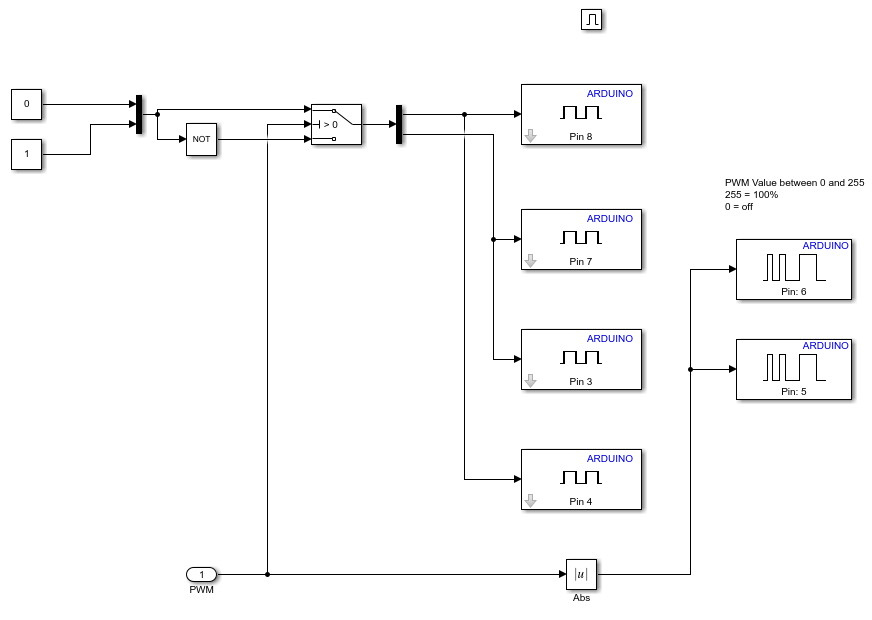
\includegraphics[width=0.7\textwidth]{figures/act.PNG}
		\caption{Converts the PWM input in direction of rotation and speedo}	
		Source: Own presentation	
		\label{fig:act}	
	\end{figure}


\section{Whole Structure}
Finally, all the blocks from the previous sections were assembled to form a single structure shown in Figure \ref{fig:struct}.

	\begin{figure}[!htbp]
		\centering
		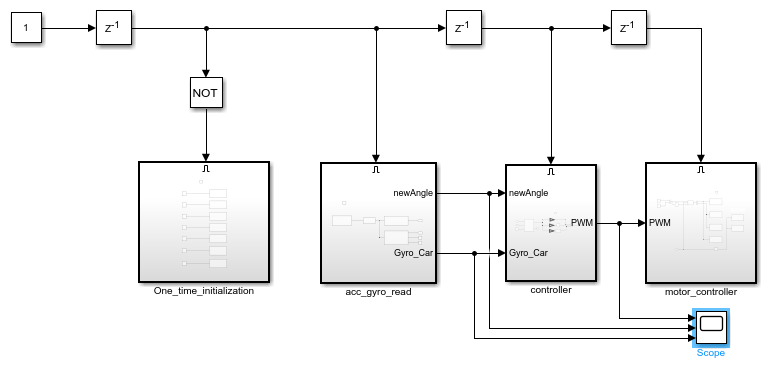
\includegraphics[width=0.7\textwidth]{figures/struct.PNG}
		\caption{The whole structure consist of blocks from the previous sections}	
		Source: Own presentation	
		\label{fig:struct}	
	\end{figure}

\section{Test with the BalanBot}
When simulating in external mode the PID controller could be adjusted. The cable did not turn out to be advantageous.
The adjustment of the PID values required a lot of patience and know-how.

\section{Conclusion}




